\documentclass{bredelebeamer}

%%%%%%%%%%%%%%%%%%%%%%%%%%%%%%%%%%%%%%%%%%%%%%%%

\title[Programación en MatLAB]{Introducción a la programación con MatLAB}
\subtitle{Módulo 02 - Variables, números y operadores}

\author{Agustín - Andrés - Gabriel - Fernando\inst{1}}
\institute[UTN.BA]
{
  \inst{1}%
  Universidad Tecnológica Nacional\\
  Facultad Regional Buenos Aires
  }

\date{2018}

\subject{Taller de programación}

\logo{

\includegraphics[scale=0.15]{images/logo.png}
}

%%%%%%%%%%%%%%%%%%%%%%%%%%%%%%%%%%%%%%%%%%%%%%%%%%%%%%%%%%%%%%%%%%%%%
\begin{document}

\begin{frame}
  \titlepage 
\end{frame}

%%%%%%%%%%%%%%%%%%%%%%%%%%%%%%%%%%%%%%%%%%%%%%%%%%%%%%%%%%%%%%%%%%%%%

% Sección variables números y operadores

%%%%%%%%%%%%%%%%%%%%%%%%%%%%%%%%%%%%%%%%%%%%%%%%%%%%%%%%%%%%%%%%%%%%%

\section{Variables, números y operadores}

\begin{frame}{Variables}
\textbf{Matlab no requiere ningún tipo de comando para declarar variables.}\\
Ej. Ejecutar las siguiente líneas. Obtener conclusiones.
\lstinputlisting[xleftmargin=.4\textwidth]{scripts/ej1.m}
\end{frame}

\begin{frame}{Variables}
\textbf{Matlab no requiere ningún tipo de comando para declarar variables.}\\
Ej. Ejecutar las siguiente líneas. Obtener conclusiones.
\lstinputlisting[xleftmargin=.4\textwidth]{scripts/ej1.m}
\begin{alertblock}{Importante}
Los nombres de las variables comienzan con una letra.
\end{alertblock}
\end{frame}

\begin{frame}{Variables}
\textbf{Matlab no requiere ningún tipo de comando para declarar variables.}\\
Ej. Ejecutar las siguiente líneas. Obtener conclusiones.
\lstinputlisting[xleftmargin=.4\textwidth]{scripts/ej1.m}
\begin{alertblock}{Importante}
Los nombres de las variables comienzan con una letra.
\end{alertblock}
\begin{alertblock}{Importante}
Matlab es sensible a mayúsculas y minúsculas.
\end{alertblock}
\end{frame}

\begin{frame}{Variables vectoriales}
\textbf{Representación de un vector de "n" elementos:}
\begin{equation*}
V = [V_1,V_2,V_3,...,V_N]
\end{equation*}
\begin{equation*}
v = [V_1 V_2 V_3 ... V_N]
\end{equation*}
\begin{columns}
\begin{column}{0.5\textwidth}
\begin{center}
Workspace\\
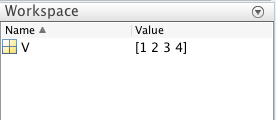
\includegraphics[scale=0.5]{images/pantalla8.png}
\end{center}
\end{column}
\begin{column}{0.5\textwidth}
\begin{center}
Command Window\\
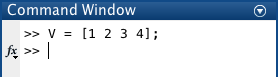
\includegraphics[scale=0.5]{images/pantalla9.png}
\end{center}
\end{column}
\end{columns}
Ej. Ejecutar las siguiente líneas. Obtener conclusiones.
\lstinputlisting[xleftmargin=.4\textwidth]{scripts/ej2.m}
\end{frame}

\begin{frame}{Variables vectoriales}
\begin{center}
\textbf{Formas de definir variables vectoriales}
\end{center}
\begin{table}[]
\centering
\begin{tabular}{|c|c|}
\hline
variable = {[}a:b{]}            & \begin{tabular}[c]{@{}c@{}}Vector cuyos primero y último elementos son a y b, \\ respectivamente. Los elementos intermedios se \\ diferencian en una unidad\end{tabular}                               \\ \hline
variable = {[}a:s:b{]}          & \begin{tabular}[c]{@{}c@{}}Vector cuyos primero y último elementos son a y b, \\ y los elementos intermedios se diferencian en la \\ cantidad s especificada por el incremento\end{tabular}            \\ \hline
variable = linespace{[}a:b:n{]} & \begin{tabular}[c]{@{}c@{}}Vector cuyos primero y último elementos son a y b, \\ y que tiene en total n elementos uniformemente \\ espaciados entre sí\end{tabular}                                   \\ \hline
variable = logespace{[}a:b:n{]} & \begin{tabular}[c]{@{}c@{}}Vector cuyos primero y último elementos son los \\ especificados y que tiene en total n elementos en \\ escala logarítmica uniformemente espaciados entre sí\end{tabular} \\ \hline
\end{tabular}
\end{table}
\end{frame}

\begin{frame}{Variables vectoriales}
Ej. Ejecutar las siguiente líneas. Obtener conclusiones.
\lstinputlisting[xleftmargin=.4\textwidth]{scripts/ej3.m}
\end{frame}

\begin{frame}{Variables vectoriales}
Ej. Ejecutar las siguiente líneas. Obtener conclusiones.
\lstinputlisting[xleftmargin=.4\textwidth]{scripts/ej3.m}
\begin{exampleblock}{Comando}
Traspuesta: \textbf{variable'}
\end{exampleblock}
\end{frame}

\begin{frame}{Variables vectoriales}
\begin{center}
\textbf{Selección de elementos de un vector}
\end{center}
\begin{table}[]
\centering
\begin{tabular}{|c|c|}
\hline
x(n)      & Devuelve el enésimo elemento del vector x                                                                                                                                                                                   \\ \hline
x(a:b)    & \begin{tabular}[c]{@{}c@{}}Devuelve los elementos del vector x situados entre el \\ a-ésimo y el bésimo, ambos inclusive\end{tabular}                                                                                      \\ \hline
x(a:p:b)  & \begin{tabular}[c]{@{}c@{}}Devuelve los elementos del vector x situados entre el \\ a-ésimo y el bésimo, ambos inclusive, pero \\ separados de p en p unidades (b\textgreater{}a)\end{tabular}                             \\ \hline
x(b:-p:a) & \begin{tabular}[c]{@{}c@{}}Devuelve los elementos del vector x situados entre el \\ b-ésimo y el a-ésimo, ambos inclusive, pero separados de \\ p en p unidades y empezando por el bésimo (b\textgreater{}a)\end{tabular} \\ \hline
\end{tabular}
\end{table}
\end{frame}

\begin{frame}{Variables vectoriales}
\begin{center}
Electrocardiograma
\end{center}
\begin{center}
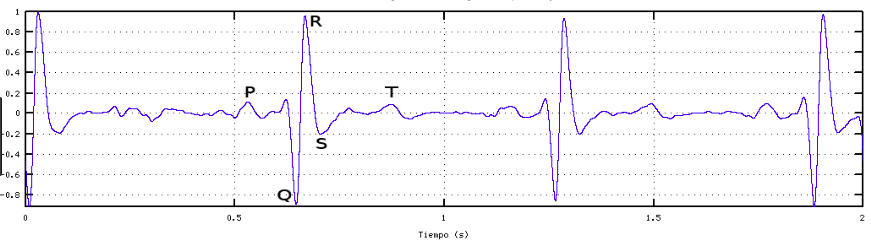
\includegraphics[scale=0.3]{images/img46.png}
\end{center}
\end{frame}

\begin{frame}{Matriciales}
\textbf{Representación de una matriz de NxM:}
\begin{equation*}
V = [V_{11},V_{12},V_{13} ; V_{21},V_{22},V_{23} ; V_{31},V_{32},V_{33}]
\end{equation*}
\begin{equation*}
v = [V_{11} V_{12} V_{13} ; V_{21} V_{22} V_{23} ; V_{31} V_{32} V_{33}]]
\end{equation*}
\begin{columns}
\begin{column}{0.5\textwidth}
\begin{center}
Workspace\\
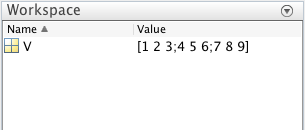
\includegraphics[scale=0.5]{images/pantalla10.png}
\end{center}
\end{column}
\begin{column}{0.5\textwidth}
\begin{center}
Command Window\\
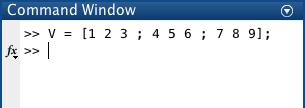
\includegraphics[scale=0.5]{images/pantalla11.png}
\end{center}
\end{column}
\end{columns}
\end{frame}


\begin{frame}{Matriciales}
\begin{center}
\textbf{Formas de definir variables vectoriales}
\end{center}
\begin{table}[]
\centering
\begin{tabular}{|c|c|}
\hline
A(m,n)         & Define el elemento (m,n) de la matriz A (fila m y columna n)                                                                                                                                                                                    \\ \hline
A(a:b,c:d)     & \begin{tabular}[c]{@{}c@{}}efine la submatriz de A formada por las filas que hay entre \\ la a-ésima y la b-ésima y por las columnas que hay \\ entre la c-ésima y la d-ésima\end{tabular}                                                  \\ \hline
A(a:p:b,c:q:d) & \begin{tabular}[c]{@{}c@{}}Define la submatriz de A formada por las filas que \\ hay entre la a- ésima y la b-ésima tomándolas de p en p, y \\ por las columnas que hayentre la c-ésima y \\ la d-ésima tomándolas de q en q\end{tabular} \\ \hline
A(a:b,:)       & \multicolumn{1}{l|}{\begin{tabular}[c]{@{}l@{}}Define la submatriz de A formada por todas las columnas de A \\ y por las filas que hay entre la a-ésima y la b-ésima\end{tabular}}                                                            \\ \hline
A(a,:)         & Define la fila a-ésima de la matriz A                                                                                                                                                                                                          \\ \hline
\end{tabular}
\end{table}
\end{frame}

\begin{frame}{Matriciales}
\begin{center}
\textbf{Matrices especiales}
\end{center}
\begin{table}[]
\centering
\begin{tabular}{|c|c|}
\hline
zeros(m,n) & Crea una matriz de m x n de ceros                                             \\ \hline
ones(m,n)  & Crea una matriz de m x n de unos                                              \\ \hline
rand(m,n)  & Crea una matriz de m x n aleatoria                                            \\ \hline
magic(m)   & Crea una matriz aleatoria especial                                            \\ \hline
eye(m,n)   & Crea la matriz de m x n con unos en la diagonal principal y ceros en el resto \\ \hline
\end{tabular}
\end{table}
Ej. Ejecutar las siguiente líneas. Obtener conclusiones.
\lstinputlisting[xleftmargin=.4\textwidth]{scripts/ej4.m}
\end{frame}

\begin{frame}{Matriciales}
\begin{center}
\textbf{Funciones sobre matrices}
\end{center}
\begin{table}[]
\centering
\begin{tabular}{|c|c|}
\hline
flipud(A) & Devuelve la matriz cuyas filas están colocadas en orden inverso    \\ \hline
fliplr(A) & Devuelve la matriz cuyas columnas están colocadas en orden inverso \\ \hline
rot90(A)  & Rota 90 grados la matriz A                                          \\ \hline
size(A)   & Devuelve el orden (tamaño) de la matriz A                          \\ \hline
tril(A)   & Devuelve la parte triangular inferior de la matriz A                \\ \hline
triu(A)   & Devuelve la parte triangular superior de la matriz A                \\ \hline
inv(A)    & Devuelve la matriz inversa de A                                     \\ \hline
\end{tabular}
\end{table}
\end{frame}

\begin{frame}{Matriciales}
\begin{center}
Ejemplo: Imagen monocromática
\end{center}
\begin{center}

\includegraphics[scale=0.3]{images/img42.png}
\end{center}
\end{frame}

\begin{frame}{Matriciales}
\begin{center}
Representación
\end{center}
\begin{center}

\includegraphics[scale=0.3]{images/img43.png}
\end{center}
\end{frame}

\begin{frame}{Matriciales}
\begin{center}
Ejemplo: Imagen color
\end{center}
\begin{center}
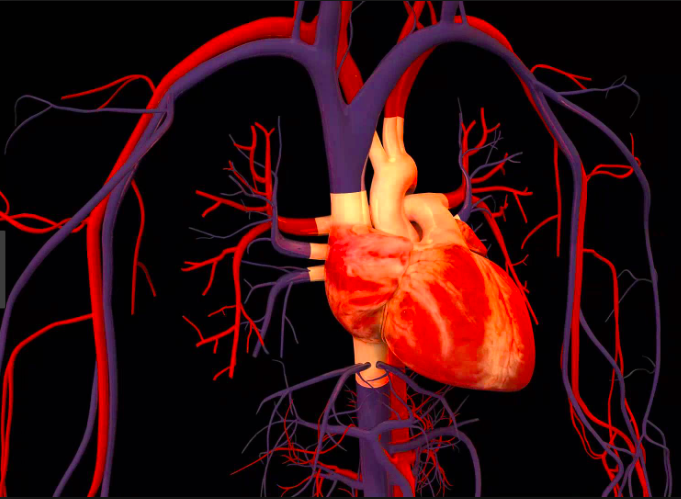
\includegraphics[scale=0.3]{images/img44.png}
\end{center}
\end{frame}

\begin{frame}{Matriciales}
\begin{center}
Representación
\end{center}
\begin{center}
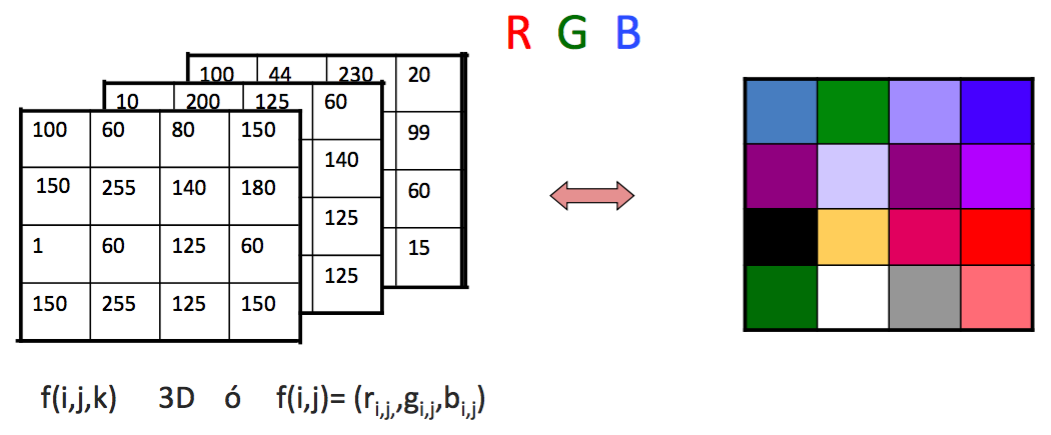
\includegraphics[scale=0.3]{images/img45.png}
\end{center}
\end{frame}

\begin{frame}{Variables carácter}
\textbf{Arreglo de caracteres incluidos entre comillas simples.}
\begin{equation*}
c = \textbf{'}cadena de caracteres\textbf{'}
\end{equation*}
\begin{columns}
\begin{column}{0.5\textwidth}
\begin{center}
Workspace\\
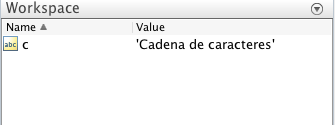
\includegraphics[scale=0.5]{images/pantalla12.png}
\end{center}
\end{column}
\begin{column}{0.5\textwidth}
\begin{center}
Command Window\\
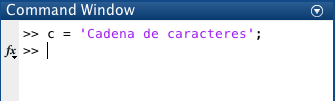
\includegraphics[scale=0.5]{images/pantalla13.png}
\end{center}
\end{column}
\end{columns}
\end{frame}

\begin{frame}{Variables carácter}
\begin{center}
\textbf{Funciones sobre caracteres}
\end{center}
\begin{table}[]
\centering
\begin{tabular}{|c|c|}
\hline
lower(‘cadena’) & Convierte la cadena a minúsculas                                                                                                                  \\ \hline
upper(‘cadena’) & Convierte la cadena a mayúsculas                                                                                                                  \\ \hline
strcmp(c1,c2)   & \begin{tabular}[c]{@{}c@{}}Compara las cadenas s1 y s2 y devuelve 1 si son \\ iguales y 0 en caso contrario\end{tabular}                           \\ \hline
strcmp(c1,c2,n) & \begin{tabular}[c]{@{}c@{}}Compara las cadenas s1 y s2 y devuelve 1 si son iguales sus n \\ primeros caracteres y 0 en caso contrario\end{tabular}                                                           \\ \hline
disp(‘cadena’)  & Muestra la cadena y continúa el proceso de MATLAB                                                                                                 \\ \hline
\end{tabular}
\end{table}
\end{frame}

\begin{frame}{Números}
\textbf{Tipos de números:}
\begin{itemize}
\item Números enteros
\item Números racionales
\item Números reales
\item Números complejos
\end{itemize}
\textbf{Operaciones permitidas con números}
\begin{table}[]
\centering
\begin{tabular}{|c|c|}
\hline
x+y                  & Suma       \\ \hline
x-y                  & Diferencia \\ \hline
x*y                  & Producto   \\ \hline
x/y                  & División   \\ \hline
x\textasciicircum{}y & Potencia   \\ \hline
\end{tabular}
\end{table}
\end{frame}

\begin{frame}{Números}
\begin{center}
\textbf{Números irracionales y reales especiales}
\end{center}
\begin{center}
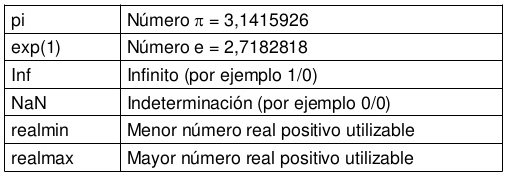
\includegraphics[scale=0.6]{images/irracionales.png}
\end{center}
\end{frame}

\begin{frame}{Números}
\begin{center}
\textbf{Números complejos}\\
\end{center}
\begin{table}[]
\centering
\begin{tabular}{|c|c|}
\hline
Función  & Significado                     \\ \hline
abs(Z)   & Módulo del complejo Z          \\ \hline
angle(Z) & Argumento del complejo Z        \\ \hline
conj(Z)  & Conjugado del complejo Z        \\ \hline
real(Z)  & Parte real del complejo Z       \\ \hline
imag(Z)  & Parte imaginaria del complejo Z \\ \hline
\end{tabular}
\end{table}
\end{frame}

\begin{frame}{Números}
\begin{center}

\includegraphics[scale=0.4]{images/img40.png}
\end{center}
\end{frame}

\begin{frame}{Ejercicio práctico 1}
\begin{enumerate}
\item Cree los siguientes números complejos:
\begin{itemize}
\item A = 1 + i
\item B = 2 - 3i
\item C = 8 + 2i
\end{itemize}
\item Cree un vector D de números complejos cuyos componentes reales son 2,4 y 6 y cuyos componentes imaginarios son -3, 8 y -16
\item Encuentre la magnitud (valor absoluto) de cada uno de los vectores que creo en el problema 1
\item Encuentre el ángulo desde la horizontal de cada uno de los números que creó en el problema 1
\item Encuentre la conjugada compleja del vector D
\item Use el operador transpuesto para encontrar la conjugada compleja del vector D
\item Multiplique A por su conjugada compleja y luego saque la raíz cuadrada de su respuesta.
\end{enumerate}
\end{frame}

\end{document}
